% Data

\section{Data sources} % (fold)
\label{sec:data_sources}

One posssible reason for non-reproducibility is using a data set for the reproduction enterprise that is actually different from the data set used in the original investigation.  The inability to reproduce the estimate of $\hat\Delta(1)=11430$ from equation~(2.5) by applying expression~(2.4) to the data in Table~1 suggests that this might be the case.

The data on which the paper is based consist of the counts of the number of ``word types\footnote{A ``word type'' is a lexicographically distinct string of characters.  Plural versions of singular nouns constitute distinct word types, as do different tenses of the same verb.  Different meanings of the same word, e.g., ``bear'' as a verb and as a noun are not distinguished; they are the same word type.}'' $n_x$ that appear in the Riverside edition of Shakespeare's complete works exactly $x$ times.  For instance, there are 14375 word types that appear on only one occasion in Shakespeare, and there are 4343 word types that appear on exactly two occasions.  These word type frequencies are displayed in Table~1 of ET for the 30688 word types that appear 100 times or fewer.  An additional 846 word types are said to appear more than 100 times each, but their exact frequencies are not supplied in the ET article.

The counts in Table~1 were taken from secondary sources, and reproducibility of the results would be enhanced if we could confirm at this remove that, for instance, there were no transcription errors in extracting data from the original sources.

The sources for these frequencies are ``based on Spevack's \citeyearpar{Spevack:1968qd} concordance and on the summary appearing in an unpublished report by J.~Gani and I.~Saunders.''  An article apparently based on the report appeared in the 1976 volume of \textit{Sankhy\=a} \citep{Gani:1976rg}.  That article contains a table that exactly reproduces the first two lines of ET's Table~1, which suggests that both ET and \citeauthor{Gani:1976rg} were both based on a common original source.  Because \cite{Gani:1976rg} does not contain the counts for $x=21$ through $100$, we surmise that either those values were contained in the unpublished technical report referred to in ET but omitted for space reasons in the published version, or that there is a third source based on \citeauthor{Spevack:1968qd} that contains those values.

Fortunately, Spevack's six-volume \textit{Concordance} resides in the University of Chicago's Regenstein Library, which I consulted in the hopes that these questions could be resolved.

\subsection{High frequency counts} % (fold)
\label{sub:high_frequency_counts}

Appendix~A in volume~6 of \citeauthor{Spevack:1968qd} lists all of the words in the Shakespearean corpus by frequency.  Starting with the most frequently used words, the word ``the'' appears 27457.  Because there is only one such word with that frequency, $x_{27457}=1$\footnote{As explained in section~\ref{sub:double_counting}, $x_{27457}$ should probably be taken to be zero, as the frequency count for ``the'' should be greater than 27457.}.  Each observed frequency is listed, followed by a list of all of the words having that frequency.  The first page of Spevack's Appendix~A, together with a more typical page, are shown in Figure~\ref{fig:appendixa}.

\begin{figure}
	\centering
	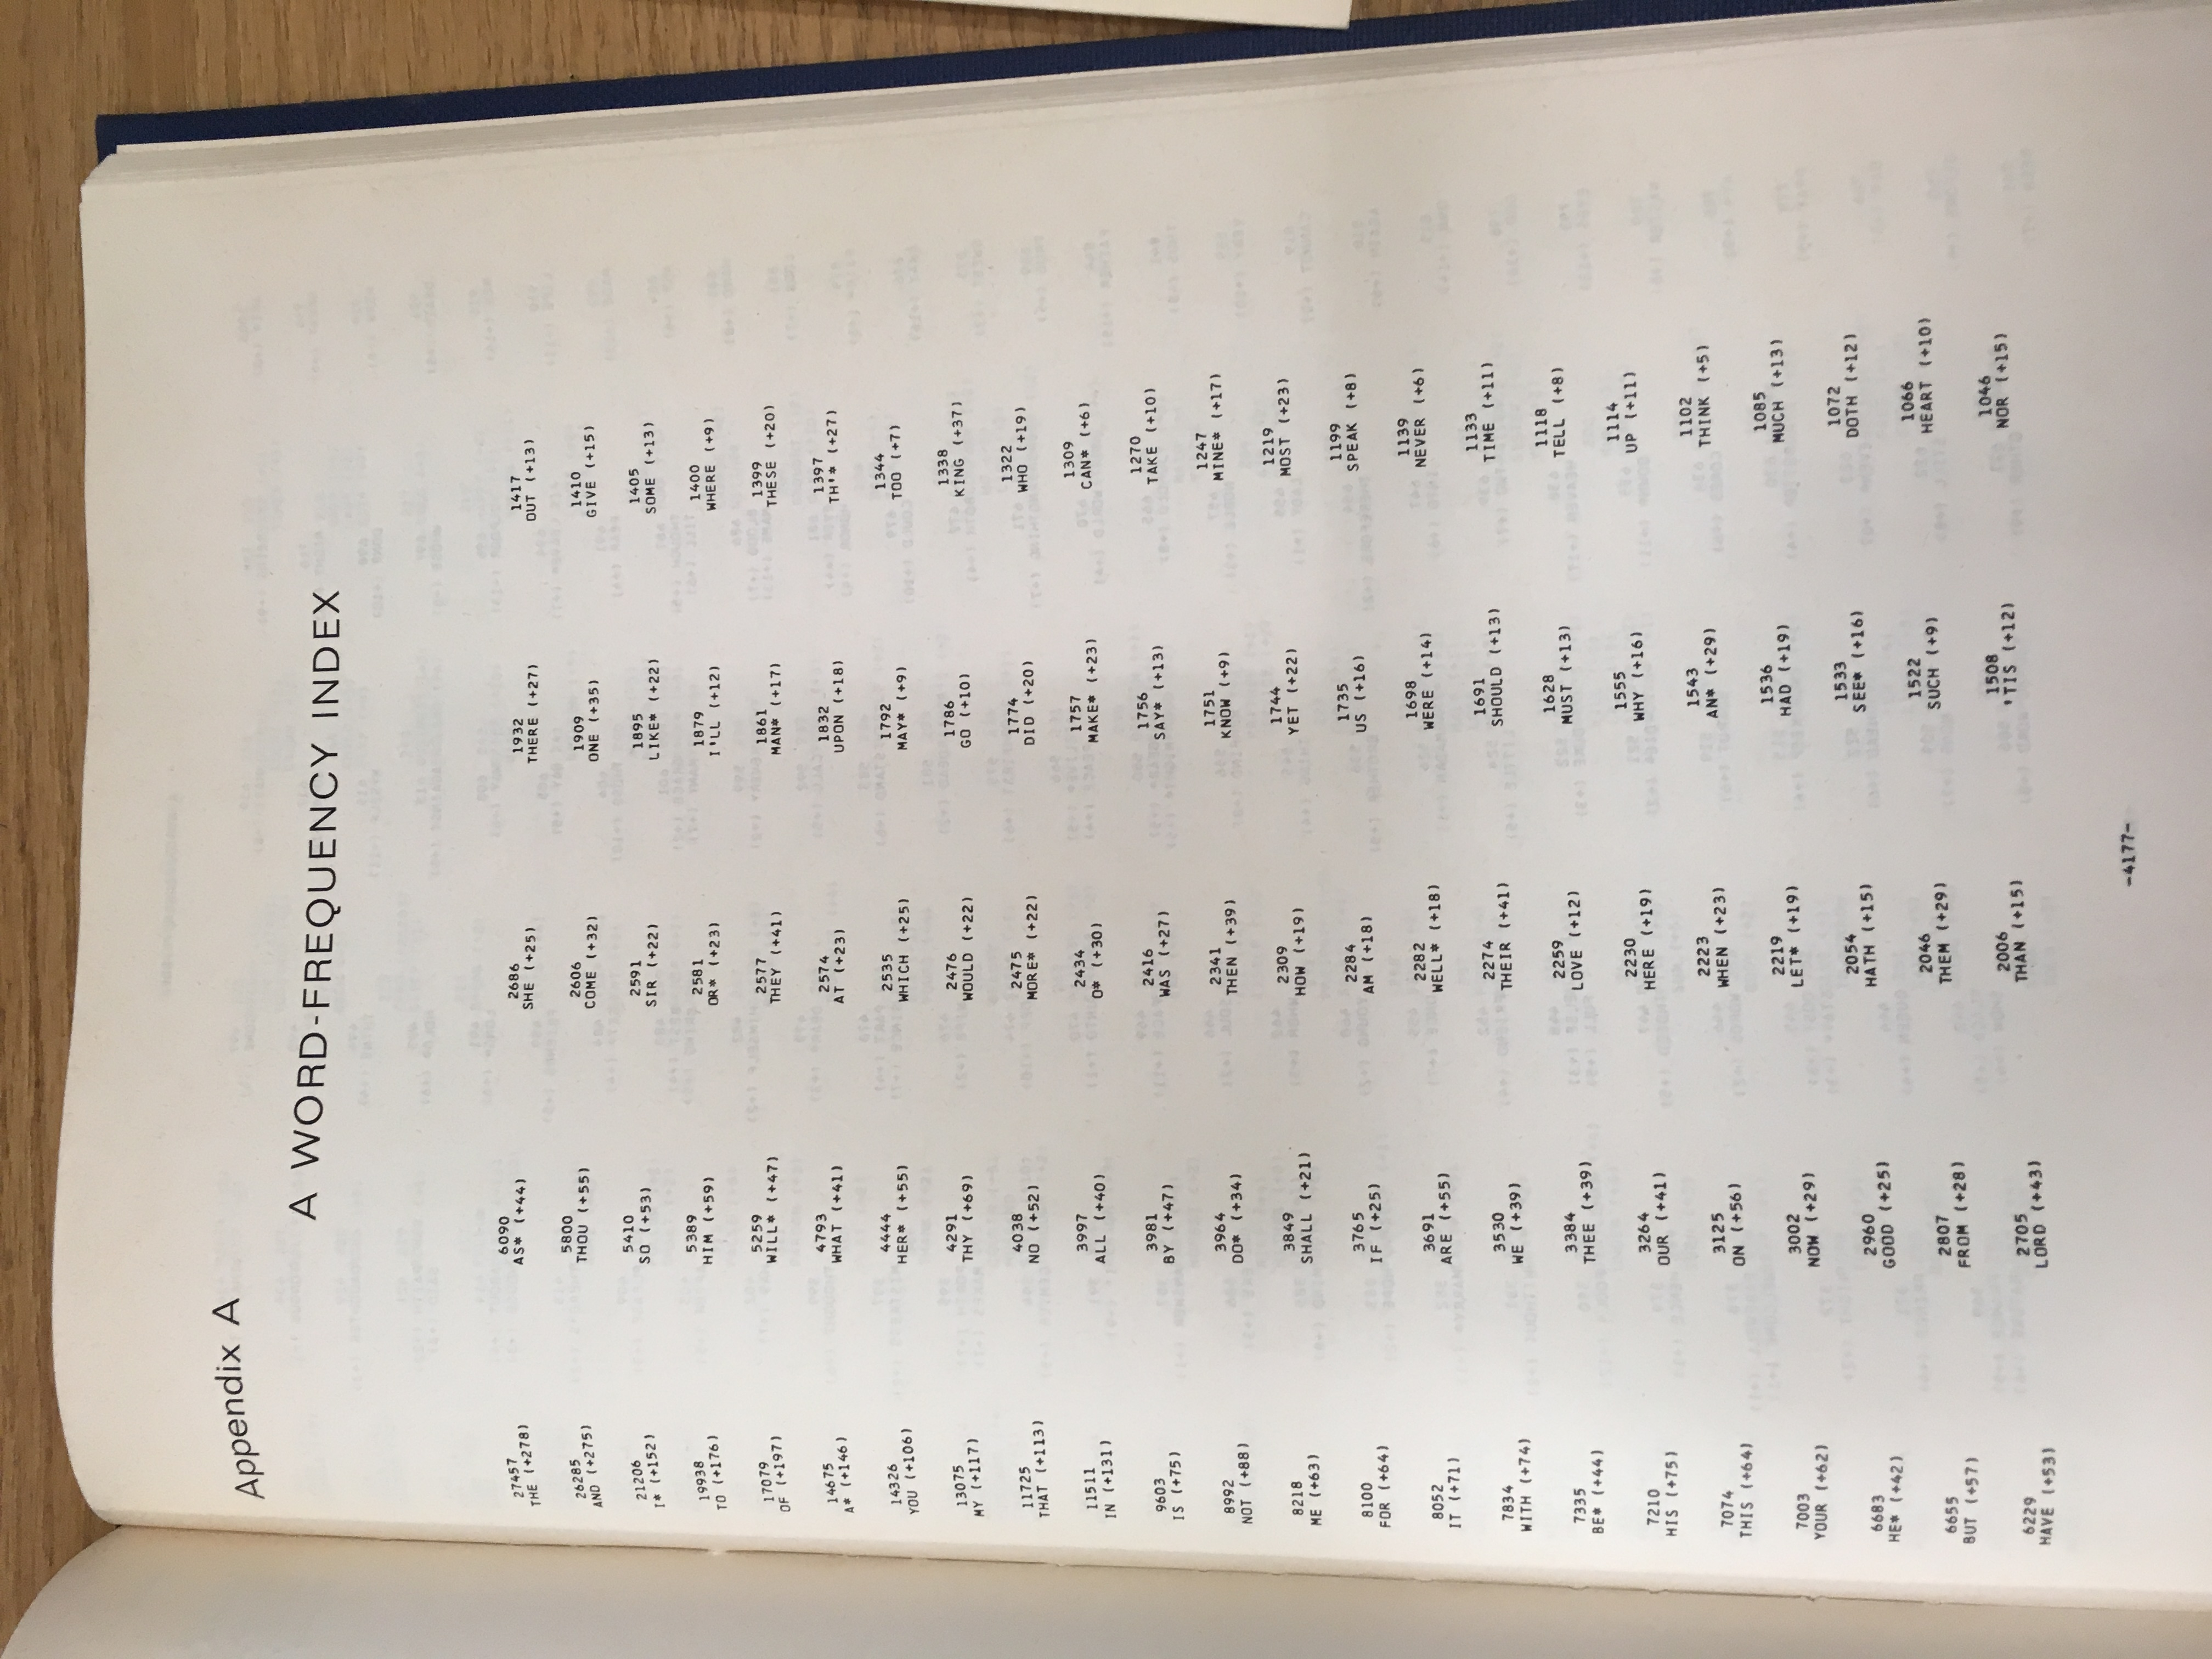
\includegraphics[width=3.25in,angle=270]{../compendium/Figures/IMG_4943.jpg}
	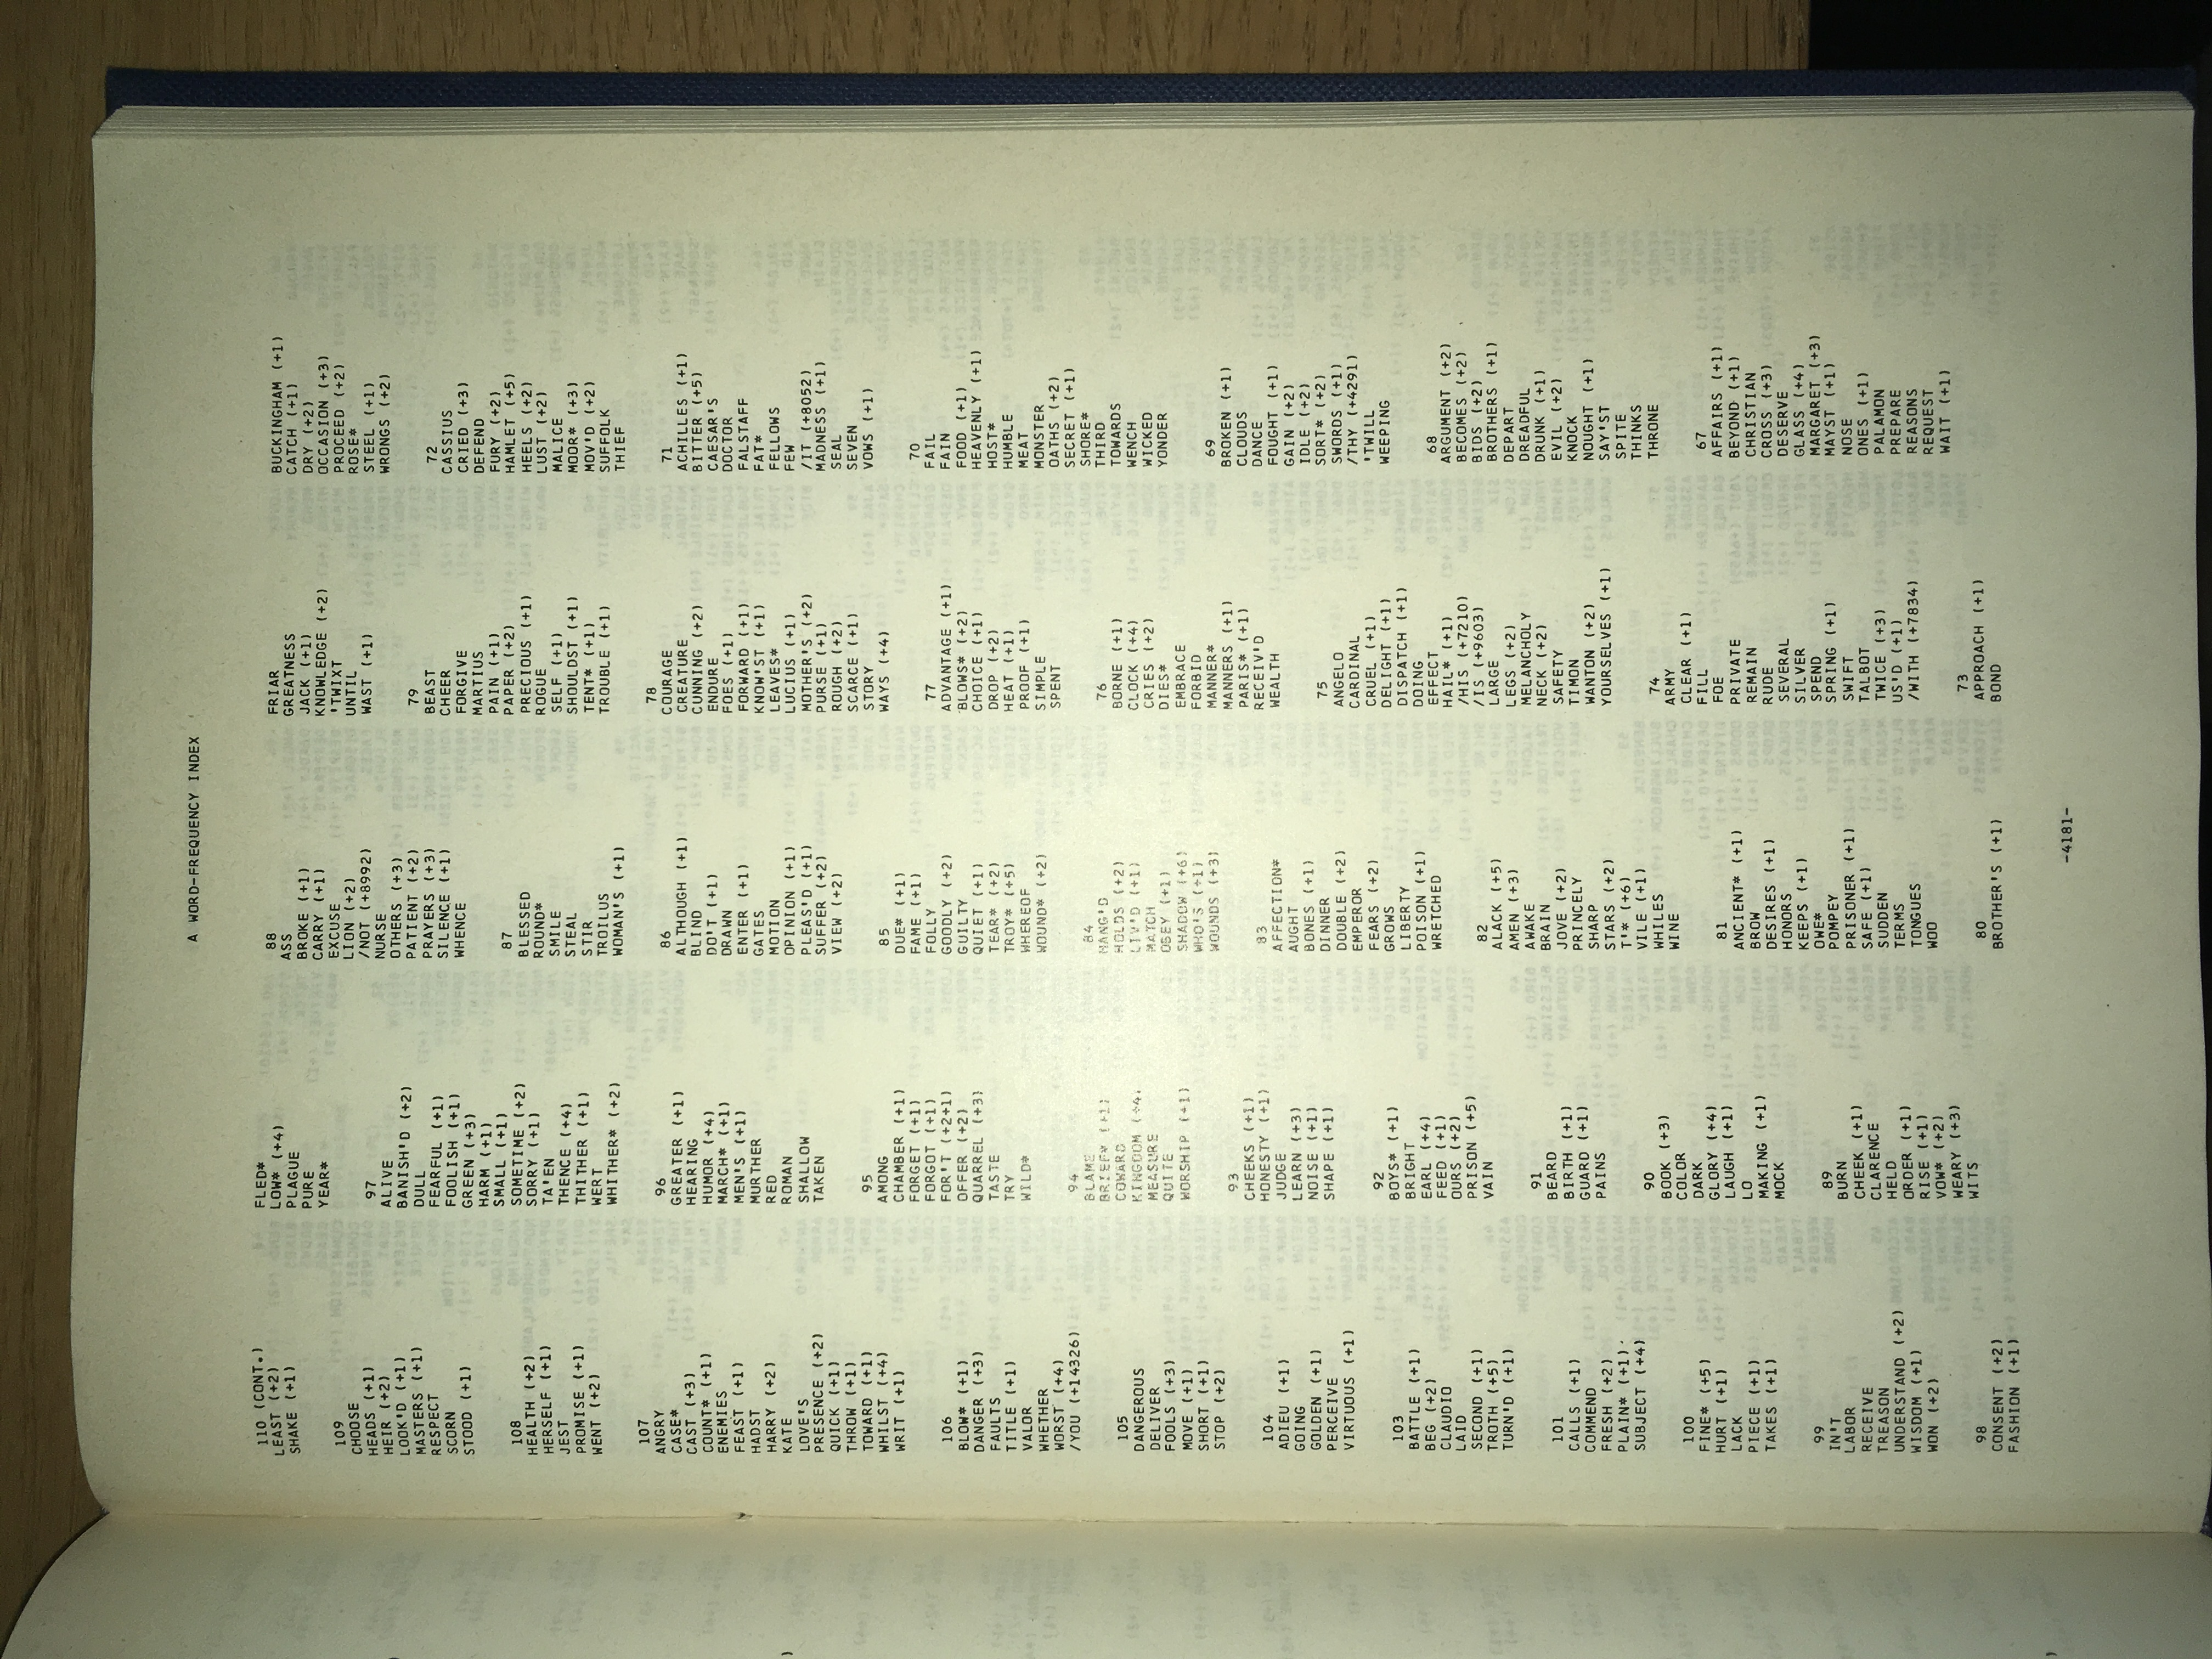
\includegraphics[width=3.25in,angle=270]{../compendium/Figures/IMG_4950.jpg}
	\caption{First page of Appendix~A in Volume~6 of \citet[p.~4177]{Spevack:1968qd}, showing very high frequency words (left), and typical page (p.~4181) showing words with frequencies 67 through 109 (right). }
	\label{fig:appendixa}
\end{figure}

Figure~\ref{fig:appendixadetail} shows detail from the right-hand display in Figure~\ref{fig:appendixa}, specifically the entries corresponding to the frequencies $x=99$ and $x=100$.  The number of words shown, $x_{99}=7$ and $x_{100}=5$ agree with the corresponding entries in Table~1 of ET.

\begin{figure}
	\centering
	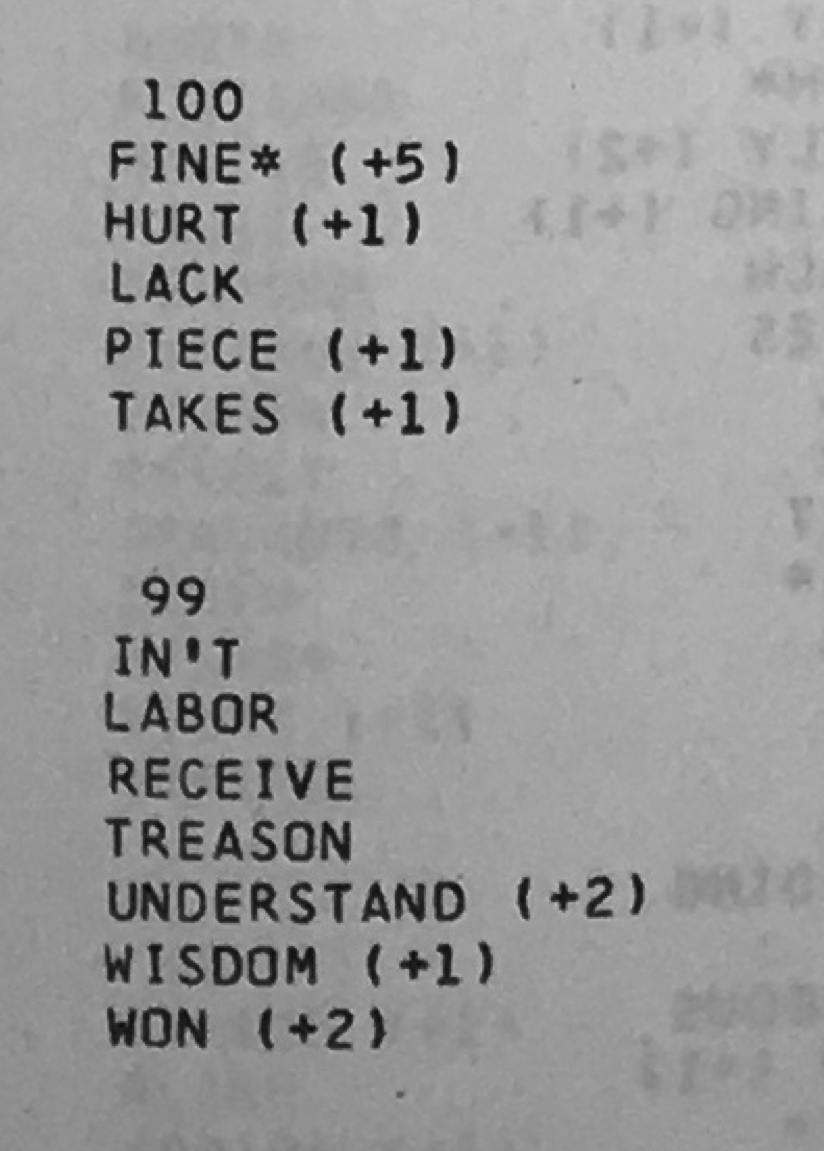
\includegraphics[height=2in]{../compendium/Figures/IMG_4950_detail.pdf}
	\caption[]{Detail from Appendix~A in Volume~6 of \citet[p.~4181]{Spevack:1968qd}, showing words that appear 99 and 100 times in Shakespeare. The asterisk appearing next to the word \texttt{FINE} indicates that the word is a homograph, that is a word type that Shakespeare used with at least two different meanings in different settings.  ``Fine,'' for instance, can be a noun indicating a penalty, a verb meaning to purify, or an adjective meaning exquisite, among many other meanings.  In any event, homographs have no affect on any of the analyses (or models) in ET.}
	\label{fig:appendixadetail}
\end{figure}

{\LARGE \color{red}\citeauthor{Efron:1976zs} report}
% subsection high_frequency_counts (end)

\subsection{Reproducing Table~1 of Efron and Thisted} % (fold)
\label{sub:et_table_1}
{\LARGE \color{red} TO WRITE UP}

% subsection et_table_1 (end)

\subsection{Double counting} % (fold)
\label{sub:double_counting}

Although Spevack reports that the most common word in Shakespeare (``the'') appears 27457 times, he also reports that it appears an additional 278 times in square brackets in the Evans edition of Shakespeare on which the Spevack \textit{Concordance} is based.  These words resulting from editorial emendation are counted as separate word types in the ET and Gani/Saunders compilation, and this is probably an error.  The bracketed words should be counted as if they were used by Shakespeare, as they constitute the best editorial asssessment of what Shakespeare wrote.  In that case, both $x_{27457}$ and $x_{278}$ are each too large by one, and $x_{27735}$ should be incremented by one).  In this case, the total number of unique words reported in ET is too large, as words that ever appear in editorial brackets are counted twice.

Figure~\ref{fig:appendixadetail} illustrates how the effect of double counting is potentially substantial. For instance, four of the five entries for $x=100$ have parenthetical counts that correspond to the number of times the same word appears in editorial brackets.  Thus, only one of the five words listed under $x=100$ appeared exactly 100 times!

An alternative way to account for bracketed words would be to say that, because they are a result of editorial rather than Shakespearean action, that they should be disregarded entirely.  In that case, $x_{27457}$ would remain at one, but $x_{278}$ should be decremented by one to account for disregarding ``[the]''.

In either case, the total number of word types reported by ET is be overstated.  Indeed, Spevack reports that the total number of unique words in the Shakespearean corpus is 29066 (Spevack, vol 4, p.~1), and this figure is echoed by Gani and Saunders. Both are at odds with the total of 31534 reported in ET.  This suggests that roughly 2500 words were counted twice.

Recalculating Table~3 and everything that follows from it to take this double counting into account would require a substantial amount of effort to identify, extract, and correct the myriad instances of this type of double counting, an effort which I may take on at a later point in time.

% subsection double_counting (end)
% section data_sources (end)

